%% LyX 2.1.3 created this file.  For more info, see http://www.lyx.org/.
%% Do not edit unless you really know what you are doing.
\documentclass[english]{article}
\usepackage[T1]{fontenc}
\usepackage[utf8x]{inputenc}
\usepackage{geometry}
\geometry{verbose,tmargin=2cm,bmargin=2cm,lmargin=2cm,rmargin=2cm,headheight=2cm,headsep=2cm}
\setcounter{secnumdepth}{3}
\setcounter{tocdepth}{3}
\usepackage{float}
\usepackage{amsthm}
\usepackage{amsmath}
\usepackage{amssymb}
\usepackage{graphicx}
\bibliographystyle{plain}
\makeatletter

%%%%%%%%%%%%%%%%%%%%%%%%%%%%%% LyX specific LaTeX commands.
%% Because html converters don't know tabularnewline
\providecommand{\tabularnewline}{\\}
\floatstyle{ruled}
\newfloat{algorithm}{tbp}{loa}
\providecommand{\algorithmname}{Algorithm}
\floatname{algorithm}{\protect\algorithmname}

%%%%%%%%%%%%%%%%%%%%%%%%%%%%%% Textclass specific LaTeX commands.
\numberwithin{equation}{section}
\numberwithin{figure}{section}

%%%%%%%%%%%%%%%%%%%%%%%%%%%%%% User specified LaTeX commands.
\usepackage{babel}

\makeatother

\usepackage{babel}
\begin{document}

\title{Modélisation, Simulation multi-niveau pour l'optimisation de politiques
de vaccination }


\author{TRAN Thi Cam Giang, Jean Daniel ZUCKER, Marc CHOISY, Yann CHEVALEYRE}


\date{03/06/2015}

\maketitle

\section{State of the art}


\subsection{Epidemiology ( and monitoring) }


\subsubsection{Epidemiology}
As we know that public health problems are one of the emerging troubles
in the entire world. They directly influence human heath, the health
of one person, the health of a community. In particular, any news
about infectious diseases for children has always been a subject of
concern to parents as well as everyone. Hence, in the world, a discipline
``epidemiology'' has risen to study the factors, causes, and effects
of infectious diseases. 

This thesis is proposed in a context in which many public health serious
events have occurred in the world : SRAS in 2003, avian influenza
in 2004 or swine flu in 2009, etc. In particular, at the
start of 2014, the World Health Organization (WHO) officially stated
global measles epidemic outbreak. In the first three months of the
year 2014, there were about 56,000 cases of measle infections in 75
countries, particularly in southeast Asia and in
Vietnam.
This has pointed out the important role of the epidemiological phenomena
anticipation when diseases occur. Many studies proposed by the WHO,
the Pasteur Institute and the Inserm in the field of environmental
security try to understand disease phenomena and spread
of disease over a territory, to better manage when diseases occur.
These researches consist of mathematical or statistical studies via
surveillance networks \cite{chauvin1994constitution}. This is one
of the axes of the UMMISCO laboratory's research themes (IRD UMI 209).


\subsubsection{Control}

Pathogenic microorganisms such as bacteria, viruses, parasites or
fungi are key factors causing infectious diseases. The diseases can
be spread directly or indirectly from one person to another, through
a mediate environment or contaminated tools. As far as directly infectious
diseases are concerned, meaninf diseases directly transmitted from
one person to another, we have some normal policies to prevent the
spread of diseases such as vaccines, anti-viral medications, and quarantine.
In this thesis, we focus on vaccines in the human community. A vaccine
is understood as a biological preparation that provides active acquired
immunity to a particular disease for our body. After having been vaccinated,
we transport microorganisms in weakened or killed form of the microbe
into our body. The body's immune system produces the right antibodies
to recognize the germs as a threat, destroy them and keep a record
of them. Because of that, when the disease occurs, our immune system
can recognize and destroy with a better chance of success any of these
germs that it later encounters. The administration of vaccines is
called vaccination. Vaccination has greatly helped human beings. The
vaccination of influenza, Human Papillomavirus (HPV) and chicken pox
have been particularly appreciated. Smallpox is a particular example.
This disease was filled people with terror during the closing years
of the 18th century. Smallpox killed an estimated 400,000 Europeans
annually and among the people that luckily survived, a third had been
blinded by the disease. However, the World Health Organization (WHO)
offcially stated the eradication of smallpox in 2011 \cite{tognotti2010SmallpoxErad,fenner2001SmallpoxErad}.
In addition, many infectious diseases are clearly restricted such
as influenza, polio, measles and tetanus from much of the world. Thus,
one big question proposed is why many infectious diseases still exist
in the world though we have produced vaccines for most infectious
diseases. In order to answer this question, first of all, we have
to answer to some following small questions :

\begin{table}[h]
\begin{tabular}{|c|c|c|}
\hline 
\textbf{Question} & \textbf{Answer} & \textbf{Why?}\tabularnewline
\hline 
\hline 
Are vaccines safe? & YES & Vaccines are generally quite safe\tabularnewline
\hline 
Are there vaccines for all infectious? & NO & For example: dengue\tabularnewline
\hline 
Are all vaccines free?  & NO & Funding problem \tabularnewline
\hline 
Are all people vaccinated before a requested age for each disease? & NO & Funding/geographic/cultural problems\tabularnewline
\hline 
\end{tabular}

\protect\caption{Vaccine state}


\end{table}


With the four answers above, we can say that the human still faces
up to infectious diseases. A thorough knowledge of the disease is
essential in order to implement large-scale proper infection control
measures and prevention campaigns. Granted that the disease transmission
methods depend on the characteristics of each disease and the nature
of the microorganism that causes it. In this thesis, we will investigate
popular infectious diseases with transmission by direct contact. This
transmission requires a close contact between an infected person and
a susceptible person, such as touching an infected individual, kissing,
sexual contact with oral saliva, or contact with body lesions. Therefore,
these diseases usually occur between members of the same household
or close friends and family. In particular, this thesis will mostly
focus on measles. Because measles is a highly contagious, serious
disease caused by a virus. It is a typical infectiuous disease with
direct transmission. In 1980, approximate 2.6 milion people was killed
each year before we had the widespread vaccination policies. It spreads
very fast by coughing and sneezing in human communities via close
interpersonal contact or direct contact with secretions. Its main
symptoms consist of high fever, cough, runny nose and red eyes. These
first symptoms usually take from 10 to 12 days after exposure to an
infectious person, and lasts 4 to 7 days \cite{panum1988observations}.
In fact, now there is no proper treatment for measles to totally prevent
the spread of measles except routine measles vaccination policy for
children. According to the report by the World Health Organization
(WHO), since 2002 measles was eradicated from U.S. However, today
measles vaccination has not been extensively popularized in the entire
world. Beside the obtained results, for example, in 2013, there was
about 84\% of the world's children having received one dose of measles
vaccine, and during 2000-2013, measles vaccination prevented an estimated
15.6 million deaths; we have had to face upabout 145700 measles deaths
globally- estimated 400 deaths every day or 16 deaths every hour in
2013. Measles becomes one of the leading causes of death among young
children in the world, although now we are having a big stock of safe
and readily available measles vaccines.

Mass policy (or the routine measles vaccination policy for measlses)
that vaccinates the maximum number of children before a certain age,
is the oldest (started from the 1950s in the rich countries) and is
now the most used. The policy has obtained clear results : a clear
decrease of the incidence in most countries. However, the problem
of this vaccination policy is too expensive, really ineffective and
quite impossible to implement in poor countries, especially in Africa
because of both financial and logistical problems. (e.g. the WHO project
``Extended Program on Immunization'' in Vietnam for the measles
extinction before 2012 failed \cite{WHOProjectEPI}). In
addition, when a vaccination policy is performed in a country, there
is only one policy deployed, but in modeling, we can realize many
policies and assess their results. 

In short, measles is still a common and often fatal disease in the
world. We still very much need to model the transmission dynamics
of measles and investigate the effect of vaccination on the spread
of measles in the entire world. More largely, we need to give new
optimal vaccination policies in artificial intelligence in order that
these policies may become more effective, less expensive, and take
into account the spatial dimension for all popular infectious diseases.


\subsection{Dynamiques/structures spatiales (théorie métapopulations, réseaux,
etc…) }
\begin{itemize}
\item For directly transmitted infectious diseases by virus and bacteria,
susceptible individuals are not only infected by infected individuals
in the same location, but also by other infected individuals due to
the movement of individuals between populated regions. This is one
very important part in the domain studying the geographical spread
of infectious diseases. We care for host population characteristics,
then characteristics of spatial spread of an infectious disease among
populations. Through these characteristics, we find optimal policies
to minimize the number of infected individuals in a community. In
fact, there are many studies about the interactions among populations.
However, we can divide the spatial structure of populations into two
main levels: ``inter-city level'' and ``intra-city level''. At
the inter-city level (or called ``micro-level''), we use differential
equations to control its models. At the ``intra-city level'' ( also
called ``macro-level'') in which we provide connections between
the populations, simulate the intra-city traffic. We consider the
effect of travel through the connections between population regions
as a means of spreading a virus \cite{shaw2010effective}. 
\item We have two basic models considered in the ``macro-level'', the
model has no explicit movement of individuals and the models describes
enough travels and movements of individuals among populations and
even takes into account the resident population as well as the current
population of individuals \cite{van2008spatial}. A population may
be simplified as a city, community, or some other geographical region.
Population travel (e.g. among animals and among people by foot, birds,
mosquitoes and in particular, people travel by air from one city to
another), is the main reason why diseases can spread quickly among
very distant cities such as SARS disease in 2003. Therefore, the term
``metapopulation'' arrived in the ecological literature in 1969
by Levins \cite{Levins1969,hanski1991metapopulation}. A metapopulation
is a population of a set of spatially discrete local populations (or
subpopulations in short) with mutual interaction \cite{Levins1969}.
In the metapopulation in which a subpopulation can only go extinct
locally and be recolonized by another after it is emptied by extinction
\cite{Bolker1996,Hanski1998,Levins1969} and migration between subpopulaitons
is significantly restricted. In a metapopulation, if recolonization
rates are smaller than extinction rates, then total extinction of
all local population will easily be reached. The persistence time
of the metapopulation is measured as the time until all subpopulations
go extinct. According to Harrison (1991) \cite{hanski1991metapopulation}
there are four types of spatially dynamic populations : classic Levins
metapopulation, mainland-island metapopualtion, patchy population
and non-equilibrium populations. 

\begin{itemize}
\item The first metapopulation model was proposed in 1969 by Levins. It
is called the classic Levins Metapopulation \cite{Levins1969}. Wilson
in 1980 \cite{wilson1980natural} stated that in this classic model
``A nexus of patches, each patch winking into life as a population
colonizes it, and winking out again as extinction occurs.''


\begin{figure}[h]
\centering
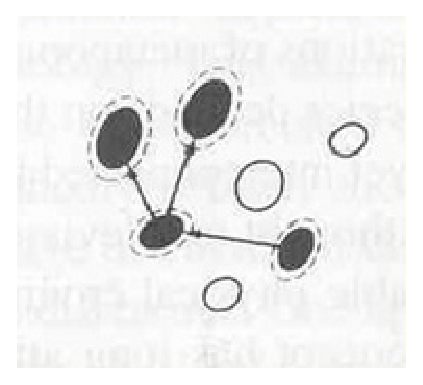
\includegraphics{classicLevinsMeta}
\protect\caption{Classic Levins Metapopulation Model \cite{harrison1997empirical}}
\end{figure}



All subpopulations in this classic model are relatively small. The
levels of interaction among individuals within a subpopulation is
much higher than between subpopulations.

\item The second model is the mainland-island metapopulation in which there
are some small ``island'' subpopulations within dispersal distance
of a much larger ``mainland'' subpopulation.


\begin{figure}[h]
\centering
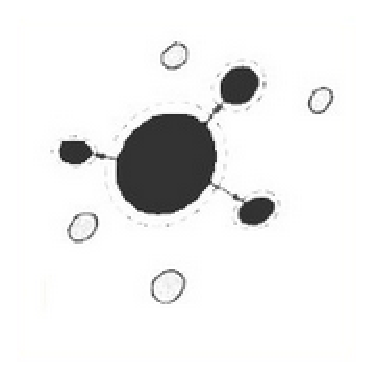
\includegraphics{mainlandIslandMeta}
\protect\caption{Mainland-Island Metapopulation \cite{harrison1997empirical}}


\end{figure}
It is evident that smaller subpopulations have a high probability
of local extinction, but the mainland population will hardly become
extinct. The migration from the mainland to the islands is independent
of the islands white or filled, but is propagated for the connected
islands. Therefore, if the mainland population has a low individual
density and there is no immigration, then population growth rate is
positive. Inversely, if island populations are in the same conditions
as the mainland, then its population growth rate is negative. Thus,
the islands would go down to extinction if there are no imemigrants. 

\item The third model is patchy population. The local populations exist
in a big habitat population and the dispersal rate between subpopulations
is high. 


\begin{figure}[h]
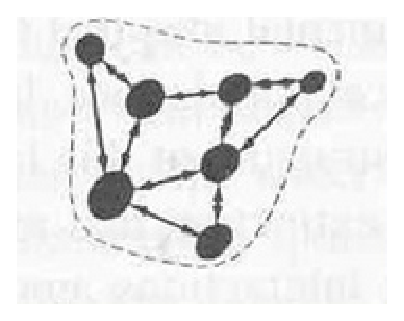
\includegraphics{figPatchyPopulation}

\protect\caption{Patchy population \cite{hanski1991metapopulation}}


\end{figure}



Here we can find that the population structure is grouped and the
interaction among them is frequent. However, this model is not referred
as a concept for metapopulation and most researchers do not consider
this a meta-population either.

\item The final model is the non-equilibrium population. The local populations
are patches, its local extinctions are much greater than its recolonisation.


\begin{figure}[h]
\centering
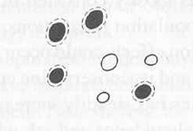
\includegraphics{figNonEquilibriumPopulation}

\protect\caption{Non-equilibrium population \cite{hanski1991metapopulation}}


\end{figure}



It is obvious that white patches are rarely or never recolonized.
Therefore, this model is not considered as a functional metapopulation.
We can find this model in forested agricultural fields.

\end{itemize}
\end{itemize}
We already have four metapopulation models. In order to model the
metapopulations mentioned above, we have three main model to implement
: spatially-implicit model, spatially-explicit model and spatially-realistic
model. For the first model, this is the type of model used in Levins
(1969) \cite{Levins1969} in which supposing that all local populations
are connected with each other and they have independent local fluctuations.
At any one time, we save track of the proportion of local populations
and we do not take care the distance between them and the population
size of each subpopulation. This model are mathematically and conceptually
easy to implement. But this model can only answer some metapopulation
problems because it ignores so many variables of a metapopulation.
This model should be used for metapopulation close to a steady state. 

For the second model, the spatially-explicit model is more complex
than the first model. Subpopulations may be filled or vacant. Local
populations only have interactions with the nearest neighbors. Subpopulations
are organized as cells on a grid and migration among them depends
on population density. We also only consider presence or absence of
a species in each subpopulation. The advantage of this model is easy
to model because of same local behaviors from subpopulation to subpopulation.
However, we cannot simply describe the state of the metapopulation
through filled subpopulations. Finally, the spatially-realistic model
uses GIS to realize attributes, geometric coordinates, etc ... to
a metapopulation. The first author using this model is Hanski in 1994
\cite{hanski1994practical}. His model was defined as the incidence
function (IF) model. This model is more realistic, and we can estimate
quantitative predictions about metapopulation fluctuation. However,
in fact, this model is very complicated, and many geographic data
have to be estimated. Hence, the metapopulation concept start to no
longer exist.

In the scope of this thesis, we focus on a metapopulation model that
is result of combination between the spatially-explicit model and
the patchy population. In general, this a simple spatial model, but
is one of the most applicable model to descrire spread of diseases
in human communities. This metapopulation consists of distinct ``subpopulation,
each of which fluctuates independently, together with interaction
limited by a coupling parameter $\rho$. These subpopulations may
be filled or empty and contact with any neighbours. 


\subsection{Epidemiologic models}

It is known that, there are many current models that are used to model
complex systems in nature, in ecology system and in epidemiology.
Mathematical models in epidemiology are a typical exemple. These models
permit us to present behavior of diseases and disease process in mathematics.
However, explaining the transmission of infectious diseases is a difficult
problem for an epidemiologist. Because there are many different interacting
factors causing the outbreak of diseases such as the environment,
the climate, the geography, the culture,...Hence, the role of the
epidemiologist is how to model the characteristics and the transmission
process of an infectious disease. Researchers have proposed compartmental
models in epidemiology by dividing the population into ``compartments''
that illustrate health states of human through individuals. These
compartmental models are called the epidemic models too. The first
benefit of these models is to model the transmission process of a
communicable disease through compartments. Then, we can predict the
properties of the disease dynamics such as the estimated number of
infected individual, the time of persistence of disease, further that
where and when we can implement vaccination policies to have both
a minimum number of vaccined individuals and the minimum number of
infected individuals in a given population. Let image that now in
your country, there is an infectious disease as measles, a baby can
be infected. According to the process of infection of disease, firstly
this baby was born, he is fine and he is not infected yet by the measles
but he may be infected in the future. We say that he belongs to the
susceptible group (in short, S). Then, his mother takes him to a supermaket,
there he see so many people, he is really infected through any way.
He starts having a high fever, he may have to pass this state from
3 days to 5 days. In this period, he is really infected but he cannot
infecte others. We say that he belong to the exposed group (in short,
E). After that, he start decreasing the temperature, but at the same
time, he begins having red rashs on the back of the ears, after a
few hours, on the head, on the neck and finally most of the body.
This period appears from five to eight days after the exposed step.
This duration is very sensible. The baby is completely infected and
he can infecte others if they see him. He belongs to the infected
group (in short, I). Finally, he passes to the final period, he comes
back good state. We say that he belongs to the recovered group with
immunity (in short, R). 

Around these four main health groups presenting the process of infection
propagation in community, there are many epidemic models proposed.
We give here the development of epidemic models by focusing on acute
infections, assuming the pathogen causes illness for a periods of
time followed by (typically lifelong) immunity. The first simplest
model is the S-I-R model created by W. O. Kermack and A. G. McKendrick
in 1927. The authors categorized hosts within groups as described
above \textbf{S}usceptible (if not yet exposed to the pathogen), \textbf{I}nfected
(if currenly infected by the pathogen) and \textbf{R}ecovered (if
they have successfully cleared the infection). From the simplest SIR
model, in order to accord each infectious disease and real property
of disease, scientists have modified it, made it different multiforme.
However, in shape of this thesis, we concentrate on the SEIR model
(as the figure \ref{fig:seirmodel}) that fit many currently infectious
diseases in the world. Each patient must pass four health steps :
susceptible stage, incubation stage, infectious stage and recovered
stage.

\begin{figure}[tbph]
\centering 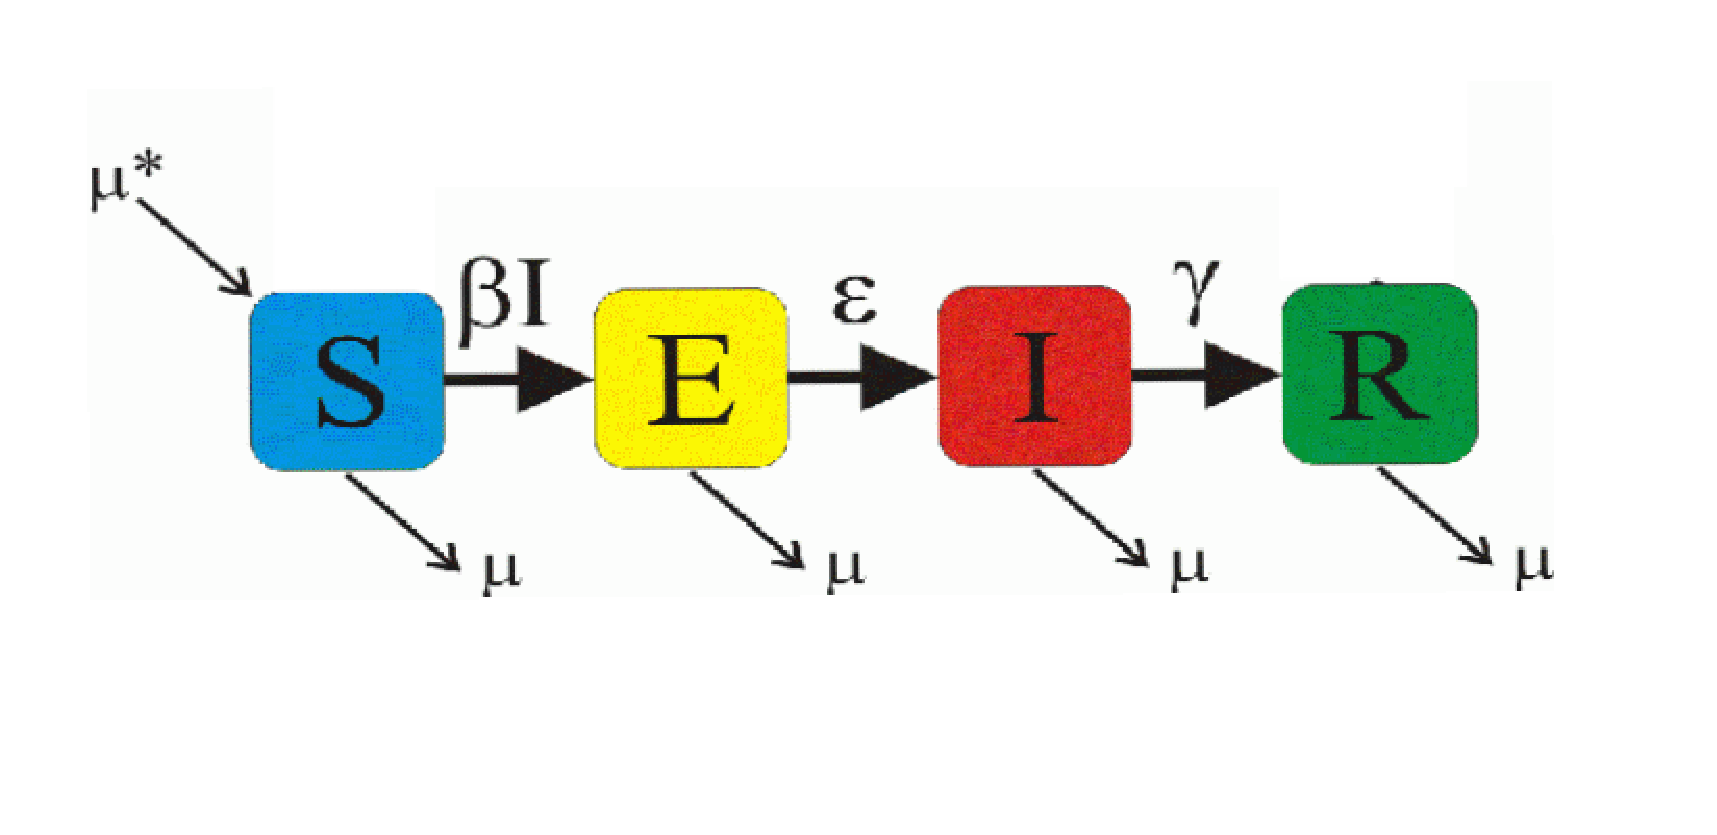
\includegraphics[scale=0.5]{seirmodel} \protect\caption{SEIR model}


\label{fig:seirmodel} 
\end{figure}


In this model, the host population (N) is divided into four classes
: susceptible S(t), exposed E(t), infected I(t) and recovered R(t).
We have :

\textbf{$N(t)=S(t)+E(t)+I(t)+R(t)$ }
\begin{itemize}
\item Classe S(t) : contains the number of individuals not yet with the
disease at time t, or those susceptible to the disease. 
\item Classe E(t) : contains the number of individuals who are in the exposed
or latent period of the disease. 
\item Classe I(t) : contains the number of individuals who have been infected
with the disease and are capable of spreading the disease to those
in the susceptible category. 
\item Classe R(t) : contains the number of individuals who have been infected
and then removed from the disease, either due to immunization or due
to death. Individuals of this classe are not able to be infected again
or to transmit the disease infection to others. 
\end{itemize}
The conceptual descriptions of the model can be represented by a flow
diagram above. The flow diagram for the SEIR model uses arrows to
present the movement between the S and I classes, the E and I classes
and the I and R classses. Here, individuals are born susceptible,
die at a rate $\mu$, become infected with the force of infection
$\lambda$ that is a function among the contact rate $\beta$, the
number of infected invidual I and the population size N, infectious
after a latency period of an average duration of $1/\sigma$ and recover
at the rate $\gamma$. 

The SEIR model is investigated by ordinary differential equations
(ODE) that are deterministic \cite{KeelingRohani2008}. The value
of variable states is only determined by parameters in the model and
by sets of previous states of these variables. Moreover, the epidemic
models are often proposed for one single population \cite{KeelingRohani2008}.
In the scope of this thesis, we propose a deterministic model for
many subpopulations in a metapopulation. The standard SEIR model (susceptible-exposed-infective-recovered)
has been strongly developed for the dynamics of directly infectious
disease \cite{Bolker1995}. For disease-based metapopulation models,
we give here a suitable new version of the SEIR equation that would
be as follows:

Consider a metapopulation of $n$ sub-populations. In a subpopulation
$i$ of size $N_{i}$, disease dynamics can be deterministically described
by the following set of differential equations \cite{Anderson&May1992}:

\begin{eqnarray}
\frac{dS_{i}}{dt} & = & \mu N_{i}-\lambda_{i}S_{i}-\mu S_{i}\label{eq:dS}\\
\frac{dE_{i}}{dt} & = & \lambda_{i}S_{i}-\mu E_{i}-\sigma E_{i}\\
\frac{dI_{i}}{dt} & = & \sigma E_{i}-\mu I_{i}-\gamma I_{i}\label{eq:infectieux}\\
\frac{dR_{i}}{dt} & = & \gamma I_{i}-\mu R_{i}\label{eq:dR}
\end{eqnarray}
 where $S_{i}$, $E_{i}$, $I_{i}$ et $R_{i}$ are the numbers of
susceptible, exposed, infectious and recovered in this sub-population
$i$ respectively. Individuals are born susceptible, die at a rate
$\mu$, become infected with the force of infection $\lambda_{i}$,
infectious after a latency period of an average duration of $1/\sigma$
and recover at the rate $\gamma$. In a case the infectious contact
rate is constant, the equilibrium values of the variables $S$, $E$,
$I$ and $R$ can be expressed analytically (see appendix). The force
of infection depends not only on the total population size $N_{i}$
and the number of infected $I_{i}$ in subpopulation $i$, but also
in other sub-populations\textbf{ \cite{KeelingRohani2008} :}

\textbf{
\begin{equation}
\lambda_{i}=\sum_{j}\rho_{ij}\kappa_{j}\log\left[1-\sum_{k=1}^{M}\left(\frac{\left|I_{k,t}\right|}{N_{k}}\times c_{ik}\times\xi_{jk}\right)\right]\label{eq:force-1}
\end{equation}
 }where\textbf{ }$c_{i,k}$ ($0\leqslant c_{ij}\leqslant1$) is the
probability that a susceptible individual native from $i$ being in
contact with another infected individual native from $k$ gets infected.
$\xi_{jk}$ ($0\leqslant\xi_{ij}\leqslant1$) refers to the probability
that an individual $y$ meeting $x$ in $C_{j}$ comes from $C_{k}$.\textbf{
}$\kappa_{j}$ is the average number of contacts per unit of time
a susceptible will have when visiting subpopulation $j$. $\rho_{i,j}$
($0\leqslant\rho_{ij}\leqslant1$) is denoted as the probability that
an individual from subpopulation $i$ visits subpopulation $j$, of
course, $\sum_{j=1}^{M}\rho_{ij}=1$. See appendix for detail on the
construction of this equation. We can verify that in the limit case
on one single subpopulation in the metapopulation ($i=j$ and $n=1$)
we have 
\begin{equation}
\lambda_{i}=-\kappa_{i}\log(1-\frac{I_{i}}{N_{i}}\times c_{ii})
\end{equation}
 Consider that the average number of contacts per unit of time $\kappa_{i}$
is seasonally forced \cite{Altizer2006} and seasonality is an annually
periodic function of time \cite{Grenfell1995}. As a result, for the
subpopulation $i$ : 
\begin{equation}
\kappa_{i}(t)=\kappa_{i0}\left[1+\kappa_{i1}\cos\left(\frac{2\pi t}{T}+\varphi_{i}\right)\right]\label{eq:beta_i}
\end{equation}
 where $t$ is the time, $\kappa_{i0}$ and $\kappa_{i1}$ are the
mean value and amplitude of the average contact rate $\kappa_{i}$
at which a susceptible will have when visiting subpopulation $i$
per unit of time, $T$ and $\varphi_{i}$ are the period and the phase
of the forcing. With the annual sinusoidal form of the average contact
rate, we really have the sinusoidally forced SEIR metapopulation model.

In detail, the deterministic model performs the same way for a given
set of initial conditions. It doesn't have randomness, dynamics, and
don't present dynamic of diseases in nature. Thus, stochastic models
have been proposed. A stochastic model is always more realistic than
a deterministic one. These models have stochastic and variable states
are not described by unique values, but by probability distributions.
It is why we will use the stochastic models to predict extinction
propability of disease in spatial context\cite{KeelingRohani2008}. 


\subsection{Algorithmes de simulation stochastique }

Stochastic simulation works on variables that both are random and
can be changed with certain probability. Today, these stochastic models
have been used widely in many domain because of some reasons as following
: before, in order to model chemically reacting systems, in simple
way, we solved a set of coupled ordinary differential equations (ODEs)
\cite{li2007stochastic}of deterministic approches. Basically, these
approches use the law of mass action that shows a simple relation
between reaction rate and molecular component concentrations. We start
with a given set of initial molecular concentrations, the law of mass
action permits us to see the component concentrations over time. The
states of a reaction are a homogeneous, free medium. The reaction
rate will be directly scaled with the concentrations of the elements.
Most systems can use the traditional deterministic approches to simulate.
It is evident that many systems such as some biochemical systems consist
of random, discreate interactions between individual elements. However,
in the case, these systems becomes smaller and smaller, the traditional
deterministic models may not be accurate. It is the reason for that
the fluctuations of these systems can be simulated exactly by applying
stochastic models, particularly as well as the Stochastic Simulation
Algorithms (SSA) \cite{gillespie1976general,gillespie1977exact}.

The SSA uses Monte Carlo (MC) methods to study the time evolution
of the jump process. Because the basis feature of the Monte Carlo
simulation is insensitive to the dimensionality of the problem, and
the work grows linearly with the number of reaction channels in the
model. The SSA describes time-evolution statistically correct trajectories
of finite populations in continuous time by solving the corresponding
stochastic differential equations. Using the stochastic models can
solve three questions. (1) These models take account the discrete
character of the number of elements and the evidently random character
of collision among elements. (2) They coincide with the theories of
thermodynalics and stochastic processes. (3) They are a good idea
to describe ``small systems'' and ``instable systems''. The main
idea of the stochastic models is that element reactions are essentially
random processes. We don't know certainly how a reaction occur at
a moment. We also call it the process stochasticity. In particular,
in the process stochasticity, we talk about demographic and environmental
stochasticities in epidemic models. The demographic stochasticity
is strongly controlled by population size such as the birth and death
rates, contamination,etc. But, the environmental stochasticity is
just affected by environmental factors what we can not govern. Therefore,
there are many epidemic models that forcus on exploration of demographic
stochasticity. Demographic stochasticity is considered as fluctuation
in population processes that are based the random nature of events
at the level of the individual. Each event is related to one baseline
probability fixed, individuals are presented in differing fates due
to chance. In addition to the demographic stochasticity, the number
of infectious, susceptible, exposed and recovered individuals is now
required to be an interger. Modeling approches that incorporate demographic
stochasticity are called event-driven methods. These methods require
explicit consideration of events. The first aprroach published by
Daniel T.Gillespie in 1976 \cite{gillespie1976general} is an exact
stochastic simulation approach for chemical kinetics. The Gillespie
stochastic simulation algorithm (SSA) has become the standard procedure
of the discrete-event modelling by taking proper value of the available
randomness in such a system. The methods modelling the event-driven
model demands explicit presentation of events. For the santard SEIR
model, we have to consider the nine events that can occur, each causing
the numbers in the relative groups to go up or down by one. Table
\ref{tab:stoch_event} lists all the events of the model, occurring
in subpopulation $i$ of a metapopulation:

\begin{table}[h]
\begin{tabular}{|c|c|c|}
\hline 
Events  & Rates & Transitions \tabularnewline
\hline 
\hline 
birth  & $\mu N_{i}$  & $S_{i}\leftarrow S_{i}+1$ and $N_{i}\leftarrow N_{i}+1$\tabularnewline
\hline 
death of a susceptible & $\mu S_{i}$  & $S_{i}\leftarrow S_{i}-1$ \tabularnewline
\hline 
death of an exposed  & $\mu E_{i}$  & \multicolumn{1}{c|}{$E_{i}\leftarrow E_{i}-1$ }\tabularnewline
\hline 
death of an infected  & $\mu I_{i}$  & $I_{i}\leftarrow I_{i}-1$ \tabularnewline
\hline 
death of an immune  & $\mu R_{i}$ & $I_{i}\leftarrow I_{i}-1$ \tabularnewline
\hline 
infection  & $\lambda_{i}S_{i}$ & $S_{i}\leftarrow S_{i}-1$ and $E_{i}\leftarrow E_{i}+1$ \tabularnewline
\hline 
becoming infectious  & $\sigma E_{i}$  & $E_{i}\leftarrow E_{i}-1$ and $I_{i}\leftarrow I_{i}+1$ \tabularnewline
\hline 
recovery  & $\gamma I_{i}$  & $I_{i}\leftarrow I_{i}-1$ and $R_{i}\leftarrow R_{i}+1$ \tabularnewline
\hline 
\end{tabular}

\protect\caption{Events of the stochastic version of the model of equations, occuring
in subpopulation $i$.}


\label{tab:stoch_event}
\end{table}


To implement this SEIR stochastic model, there are many different
methods, thought most researchers often use the method of Gillespie
in 1977. Starting from the initial states, the stochastic simulation
algorithms simulate the trajectory in population processes by repeatedly
answering the following two questions and updating the states.
\begin{itemize}
\item When (time $\tau$) will the next reaction fire?
\item Which (reaction channel index $\mu$) reaction will fire next?
\end{itemize}
So the key parameters in the SSA model are $\tau$ and $\mu$. To
calculate these distributions, we set $a_{0}(x)=\sum_{j=1}^{M}a_{j}(x)$.
The time $\tau$, given $X(t)=x$, that the reaction will fire at
$t+\tau$, is the exponentially distributied random variable with
mean $\frac{1}{a_{0}(x)}$,

\begin{align*}
 & P(\tau=s)=a_{0}(x)exp(-a_{0}(x)s),\\
\end{align*}
\label{eqProbTau}

and the index $\mu$ is the integer random variable of that firing
reaction with probability :

\begin{align*}
 & P(\mu=j)=\frac{a_{j}(x)}{a_{0}(x)}\\
\end{align*}
\label{eqProbMu}

In each step, the SSA generates random bumbers and calculates $\tau$
and $\mu$ according to the probability distribution \ref{eqProbTau}
and \ref{eqProbMu}. Below we will show some methods that simulate
exactly stochastic models. In this part, we will review the variant
formulations of Gillespie's stochastic simulation algorithm (SSA)
about the overview and the computational cost of each algorithm, then
approximate simulation methods, and finally hybrid and multi-scale
methods. We will also point out which algorithm that is most efficient,
which algorithm that we have used in this thesis.


\subsubsection{Exact stochastic simulation}

The key property for a discrete event simulation of a Markovian system
basically samples a time for the next event from this distribution
and selecting the reaction that occurs at that time. The Markovian
simulation methods have the basic steps of the widely used kinetic
Monte Carlo (KMC) method. First persons introduced the method (also
known as the KBL algorithm) are Young and Elcock in 1966 \cite{young1966monte}and
independently Lebowitz, Bortz and Kalos in 1975 \cite{bortz1975new}.
However, Gillespie really is the person who made kinetic Monte Carlo
popular in the chemical and biochemical domains, calling the algorithm
the Stochastic Simulation Algorithm (SSA) in his seminal articles
\cite{gillespie1976general,gillespie1977exact}. Below we will review
his two papers.
\begin{enumerate}
\item First reaction method (FRM) {[}GILLESPIE 1976{]} \cite{gillespie1977exact}:


The first reaction method was proposed by Gillespie in 1976. It models
demographic stochasticity in the more intuitive and slower way to
the deterministic model. The obtained result is ``fluctuations in
population processes that arise from the random nature of events at
the level of the individual'' \cite{KeelingRohani2008} The following
pseudo-code provides a clean implementation of Gillespie's first reaction
method :


\begin{algorithm}[h]
0. Labell all species $X_{1},...,X_{k}$.

1. Label all possible events $E_{1}$,...,$E_{n}$.

2. For each event determine the rate at which it occurs, $R_{1}$,...,$R_{n}$.

3. \textbf{While} $(t<t_{end}$ and $R_{N}=\sum_{v=1}^{n}R_{v}\neq0)$
\textbf{then}

4. \textbf{For} $ $$m=1,n$ \textbf{do}

5. Generate one random number $U(0,1)$ : $RAND_{m}$ 

6. At the event $m$ calculate the time until the next event is $\delta t_{m}=\frac{-1}{R_{m}}log(RAND_{m})$ 

7. \textbf{end for}

8. Find the event, $p$ , that happens first (has the smallest $\delta t$)

9. The time is now updated, $t\rightarrow\delta t_{p}$

10. Update $\{X_{i}\}$ following the event $p$.

11. Return to Step 3.

\protect\caption{Gillespie's first reaction method in 1976 - MONOPOPULATION}
\end{algorithm}



If supposing that generate one random number takes $C_{rand}$ time.
Then the FRM takes $nC_{rand}$ time per step. It is a big problem
for that Gillespie proposed a new improved algorithm in 1976. The
FRM has three main disadvantages : (1) generating random numbers is
relatively slow, (2) the FRM generates a cycle too many random numbers
in the case where the simulation time is big and the random number
generator will have tend on saturation when it generates too many
numbers, (3) the FRM is difficult for indexing the events to effectively
implement the update step.

\item Direct method (DM) {[}GILLESPIE 1977{]} \cite{gillespie1976general}
:


The Direct Method was proposed by Gillespie in 1977. The main objective
is to present the stochastic simulation for chemically reacting systems.
The following pseudo-code of this method is :


\begin{algorithm}[h]
0. Labell all species $X_{1},...,X_{k}$.

1. Label all possible events $E_{1}$,...,$E_{n}$.

2. For each event determine the rate at which it occurs, $R_{1}$,...,$R_{n}$.

3. \textbf{While} $(t<t_{end}$ and $R_{N}=\sum_{v=1}^{n}R_{v}\neq0)$
\textbf{then}

4. \textbf{For} $ $$m=1,n$ \textbf{do}

5. Calculate $R_{m}$ and $R_{m}=\sum_{v=1}^{m}R_{v}$

6. \textbf{end for}

7. Generate uniformly distributed random numbers $(r_{1},r_{2})$

8. Determine when $(\tau=ln(1/r_{1})/R_{N}$ and which $(min\{p|R_{p}\geq r_{2}R_{N}\})$
reaction will occur 

9. Set $t=t+\tau$

10. Update $\{X_{i}\}$

11. Return to step 3

\protect\caption{Direct method of Gillespie in 1977 - MONOPOPULATION \cite{gillespie1976general}}
\end{algorithm}



We can find that on each step, the Direct Method has to generate two
random numbers. Supposing that generate one random number takes $C_{rand}$
time. Hense, on each step, the DM takes $(2C_{rand}+O(n))$ where
$O(n)$ is time to search the index $p$ of the next reaction channel.
For this reason, the DM is more efficient than the FRM. 


The Gillespie algorithm plays an very important role and has become
a fundamental method in computational systems biology. Hence, many
efforts have been proposed to improve its efficiency. The key step
in the DM is to choose the next reaction channel to implement. This
step applies a linear search with a complexity $O(n)$ where $n$
is the number of occurred event in the system. Many methods have focused
on this step to improve and give more efficient formulations. For
example, Maksym in 1988 \cite{maksym1988fast} separated the set of
reactions into subsets with a complexity of $O(n^{1/2})$. In 1995,
Blue et al. \cite{blue1995faster} extended the division approach
of Maksym, where a $K-level$ method results in a search time proportional
to $n^{1/K}$. Then, in taking K to the limit, they applied a binary
tree structure and obtained the complexity $O(logR)$. Don't stop
improving, the Next Reaction Method (NRM) by Gibson and Bruck is more
known to the systems biology domain \cite{gibson2000efficient}.

\item Next Reaction Method (NRM) {[}GIBSON2000{]} \cite{gibson2000efficient}


In 2000, Gibson and Bruck successful tranformed the algorithm FRM
into an equivalent but more efficient new structure. The Next Reaction
Method applies just a sigle random number per iteration. Moreover,
the initiation times of the reactions can be set as the firing times
of independent, unit rate Poisson processes with internal times given
by integrated propensity functions. It is evaluated steady faster
than the FRM and more efficient than DM in special cases as the system
includes many species and loosely coupled reaction channels. The NRM
is presented as follows :


\begin{algorithm}[h]
1. Initialize 
\begin{enumerate}
\item set initial numbers of species, set $t=0$, generate a dependency
graph $G$
\item calculate the propensity function $R{}_{j}(x)$, for all $j$
\item for each $j$, generate a putative time $\tau_{j}$ according to an
exponential distribution with parameter $R_{j}(x)$
\item store the $\tau_{j}$ values in an indexed priority queue $P$
\end{enumerate}
2. Let $\mu$ be the reaction whose putative time $\tau_{\mu}$ stored
in $P$ is least. Set $\tau=\tau_{\mu}$

3. Update the states of the species to reflect execution of reaction
$\mu$. Set $t=\tau$

4. For each edge $(\mu,\alpha)$ in the dependency graph $G$
\begin{enumerate}
\item update $R_{\alpha}$
\item if $\alpha\neq\mu$, set


$\tau_{\alpha}=R_{\alpha,old}/R_{\alpha,new}(\tau_{\alpha}-t)+t$

\item if $\alpha=\mu$, generate a random number $r$ and compute $\tau_{\alpha}$
according to an equation similar to Step 8 of the DM


$\tau_{\alpha}=\frac{1}{R_{\alpha}(x)}log(\frac{1}{r})+t$ 

\item replace the old $R_{\alpha}$value in P with the new value.
\end{enumerate}
Go to step 2.

\protect\caption{Next Reaction Method (NRM) {[}GIBSON2000{]}}
\end{algorithm}



The data structure presented in the NRM is a dependency graph. Because
a propensity function $R_{j}$ should be modified when a given reaction
is implemented. A node in the graph is correspondent to a reaction
channel. A directed edge of the reactions $A_{i}$ and $A_{j}$ points
out that the execution of $A_{i}$ really affects the molecules in
$A_{j}$. Due to the the dependency graph, in step 4, the number of
propensity functions recalculated is minimal.


In addition, the indexed priority queue is similar to a heap tree
in computer science. It is a tree that includes ordered pairs of the
form $(i,\tau_{i})$, where $i$ is both the reaction channel index
and the position in the tree, $\tau_{i}$ is the corresponding time
when the new $A_{i}$ reaction is expected to occur. In the tree,
the value $\tau$ of each parent is a smaller than that of its children.
The top node of the tree is always the minimum value of $\tau$ and
the order is only vertical. In each step, the nodes of the tree will
change its positions according to its value to get the new prority
queue.


In short, the NRM solved two additional optimizations : (1) by switching
to absolute time, Gibson and Bruck reduced the number of random numbers
needed in each step from two to one; (2) because of the use of a dependency
graph, the number of propensities needing to be recomputed for every
timestep is minimum. In estimating the computation time of the NRM,
we find that, for every reaction channel, the time until that reaction
occurs is computed, maintained in an indexed priority queue, and efficiently
implemented as a binary heap. However, the cost for maintaining the
priority queue is relatively high. The time to select the next event
is done in constant time, but the time to update the propensities
is done in logarithmic time. Hence, the NRM is commonly used for systems
with many reaction channels and where relatively few propensities
change with each reaction. The disadvantage of the NRM is that diffusion
is added to the models and the reaction-diffusion master equation
is simulated, so systems arise. For such models, in 2004, Elf et al.
\cite{elf2004spontaneous} proposed a variant of the NRM that is called
the Next Subvolume Method (NSM). This method can be referred as a
clever association of the ideas of NRM and Maksym's method for intracellular
3D chemical reaction systems.

\item Compare the direct method (DM) to the next reaction method (NRM),
which algorithm is most efficient?


We find that in the NRM, after the executed first initial step, all
sequent timesteps only ask one random number to be generated while
the DM requests two. Even, the search step for the index $\mu$ of
the next reaction channel takes $O(M)$ time for DM, but the corresponding
task of updating the indexed priority queue takes $log(M)$. It is
the reason for that the NRM is always evaluated more efficient for
large scale problems. To evaluate the real cost of two methods (NRM
and DM) based on the total simulation time, Yang Cao et al. \cite{Cao2004}
made experiments for both formulations of SSA on a 1.4 GHz Pentium
IV Linux workstation. The problem used in their experiments is a stochastic
model of the heat shock response of E. Coli \cite{kurata2001feedback},
which includes 28 variables and 61 reactions. The experimental resultats
pointed out that the average simulation time for DM is larger than
that for NRM due to its data structure maintenance. In particular,
for the loose coupling system where the components (or elements) in
a system are interconnected and dependant on each other to the least
extent practicable, NRM works better than DM. Yang et al. found that
three main factors that strongly affect the CPU cost, are the costs,
$C_{p}$ to calculate $M$ propensities, $C_{a_{0}}$to calculate
the sum of all propensity probabilities, and $C_{s}$ to search for
a event $\mu$. Hence, to reduce these costs, Yang et al. \cite{Cao2004}
suggested that a new optimization called the Optimized Directed Method
(ODM). They found that in a reaction set of a system, some reactions
fire much more frequently than others. To reduce the search time $C_{s}$,
they arranged the index of the reaction ordering, placing the most
frequently occurring events first based on how often they fire, combined
with a dependency graph, achieves better results than the NRM for
moderately large systems. Their optimized direct method (ODM) gives
a new search depth smaller than the original method DM. The obtained
result is that $C_{s}$ can be significantly declined. In the next
step to reduce the costs $C_{a_{0}}$ and $C_{p}$, the authors used
an idea from the method NRM. The ODM only recomputes the propensities
for those reaction channels affected by the last reaction. Because
of an extra cost used for accessing the dependency graph, so this
approach applies only to loose-coupling systems. In conclusion, the
obtained results of Yang et al. have shown that the ODM is faster
than NRM, in particular, unless the system is very nearly uncoupled.
This result broken the held belief for a long time that NRM was the
fastest. 


Through this result, we can say that the efficience of the ODM, currently
is evaluated to be the fastest known algorithm for stochastic simulation
for most biological problems. This method can be negatively impacted
by transient shifts in the frequency at which reactions occur, and
commonly used in biochemical reaction networks because of the inductive
and repressive nature of genetic regulation. Due to these shifts,
the ODM defeats the pre-simulation strategy employed within the ODM
to decrease the time complexity of the SSA's reaction selection step
and thus degrade performance. In order to decrease this degradation,
in 2005, McCollum et al. \cite{mccollum2006sorting} introduced the
sorting direct method (SDM) that improves on ODM. This method eliminates
the pre-simulations required by the ODM and permits the simulator
to adapt to sharp changes in reaction execution frequencies. The common
point of these two methods is to focus on the optimization of the
system instead of the method itself by reducing the average number
of operations required to obtain the index of the next reaction to
fire. This average number of operations is called the search depth
that is hightly dependent on the biochemical system. For these two
methods, the search depth us $O(M)$. Besides, within the paper of
McCollum et al. \cite{mccollum2006sorting}, the authors also gave
a detailed overview of the difference in the implementation of DM,
NRM, ODM and SDM. In 2006, Li and Petzold introduced an alternative
formulation of the SSA, named the Logarithmic Direct Method (LDM).
In this method, the computational cost is independent of the ordering
of the reactions and no need for a pre-simulation. The LDM declined
the search depth to $O(logM)$, and pointed out the efficiency of
the logarithmic method.


Two years later, in 2008, a different approach is proposed by Hellander
\cite{hellander2008efficient} where the authors used the uniformization
and quasi-Monte Carlo to reduce the number of trajectories needed
to compute an approximation of the probability density function (PDF)
at the price of a higher cost per trajectory. Another is also found
to reduce the number of simulation in \cite{lecot2004quasi}.

\end{enumerate}
A new search direction is very beneficial to generate ensembles of
trajectories in parallel. Because the parallelization of a single
trajectory is very hard. Apply clusters to implement SSA is proposed
by Li \cite{liStochKit}. Then, Li et al. continued executing SSA
on the graphics processing unit \cite{li2007stochastic,li2010efficient}. 


\subsubsection{Approximate methods}

As mentioned above, the methods Direct, First Reaction and Next Reaction
are all exact stochastic approaches of the underlying ordinary differential
equations. Their advantage give us a really mathematically exact approach
to simulate time-to-event model (in condition that the definition
of the propensity functions accurately reflects the dynamics of the
system). But, their disavantages are 1) noise in exact simulations
only affects the probabilities associated with fates of individuals
and the updating of each consecutive event is independent – there
is no assumption concerning environmental stochasticity; 2) these
exact solutions become too slow and impractical when any one transition
rate is large, when there is a big number of subpopulations or one
a big number of event in a metapopulation; because the exact algorithms
SSA must proceed one reaction at a time and take the task of explicitly
simulating each and every reaction event, hence they are much too
slow for most practical problems. It is the reason for that, approximate
models have been proposed instead of the exact stochastic methods.
The approximate approaches ask the question : ``How many times does
each action channel fire in each subinterval?''

These approaches could be used in larger systems, and made much faster
than the exact methods. However, the exact structure of the Markov
chain is no logner simulated in the approximate approaches, hence
the validity of the approximations become a main issue. Now we will
show some mostly used approximate methods. 
\begin{enumerate}
\item $\tau-leaping$ method


Gillespie (2001) \cite{gillespie2001approximate} has proposed a new
method that decreases the simulation accuracy, but speeds up the stochastic
simulation. This is the explicit Poisson $\tau-leap$ method known
as an approximate method reduces the number of iterations by treating
transition rates as constant over time periods for which this approximation
leads to little error \cite{KeelingRohani2008}. The $\tau-leap$
method applies a Poisson approximation to can ``leap over'' many
fast reactions and approximate the stochastic behavior of the system
very well. The $\tau-leap$ method is described as follows :


\begin{algorithm}
1. Let $\delta t$ be the time increment between steps, $\delta t$
is fixed as a constant.

2. Let $M_{T}(t)$ and $M_{R}(t)$ be the number of transmission and
recovery events by time $t$.

3. Setting $\delta M_{i}=M_{i}(t+\delta t)-M_{i}(t)$ $i=T,R)$, then

\begin{align*}
 & P(\delta M_{T}=1|X,Y) & = & \frac{\beta XY}{N}\delta t+o(\delta t)\\
 & P(\delta M_{R}=1|Y) & = & \gamma Y\delta t+o(\delta t)
\end{align*}


These two equations represent the transition probabilities for transmission
and recovery events occurring in the time interval $\delta t$.

4. For small $\delta t$, the increments $\delta M_{i}$ are approximately
Poisson, such that:

\begin{align*}
\delta M_{T} & \approx & Poisson(\frac{\beta XY}{N}\delta t)\\
\delta M_{R} & \approx & Poisson(\gamma Y\delta t)
\end{align*}


5. Updating the values of the variables :

\begin{align*}
X(t+\delta t) & = & X(t)-\delta M_{T}+\delta M_{R}\\
Y(t+\delta t) & = & Y(t)+\delta M_{T}-\delta M_{R}
\end{align*}


6. Updating the time, $t=t+\delta t$.

7. Return to Step 4.

\protect\caption{$\tau-leap$ method proposed by Gillespie (2001)\cite{KeelingRohani2008}}
\end{algorithm}



The main problem in the $\tau-leap$ method is relative to the value
of the time increment between steps, $\delta t$. How do we choose
the value fixed of $\delta t$? $\delta t$ must satisfy two conditions,
large enough so that many reaction events occur in that time and small
enough of the leap condition. The leap condition is pointed out that
\cite{cao2007adaptive}: For the current state $x$, the value of
$\delta t$ is asked to be small enought that the modification in
the state during $[t,t+\delta t]$ will be so small that no propensity
function will suffer an appreciable change in its value. Thus, the
key to the success of this technique is to choose a leap size large
enough to allow many reactions to occur during the leap (reducing
computation) and small enough that none of the propensity functions
will change significantly in value (causing an error). Cao et al.
\cite{cao2005avoiding} pointed also out a method to estimating the
largest value of $\delta t$, the expected change in each propensity
function during a leap be limited by $\epsilon a_{0}(x)$, where $\epsilon$
$(0<\epsilon\ll1)$ is the error control parameter. In short, the
best advantage of the $\tau-leap$ method is to speed up the stochastic
simulation for many ``not-too-stiff'' systems $-$i.e., systems
in which the difference between the characteristic time scales of
the fastest and slowest dynamical modes is not too large. However,
the number of firings of each reaction channels during a fixed time
step $\delta t$ is approximated as a Poisson random varibale. This
Poisson variable can have arbitrarily large sample values. Hence,
there exists the possibility that this $\tau-leap$ method will cause
one or more reaction channels to fire so many times during $\delta t$
that number of reactants in each population will be became negative,
in particular in systems with multiple timescales (for short the stiff
systems). Due its obtained advantage, so this technique has continued
to mature, specially in the area of leap-size selection, through the
work of a variety of researchers : procedure for determining the maximum
leap size for a specified degree of accuracy \cite{gillespie2003improved};
a binomial leaping method developed independently Tian et al.\cite{tian2004binomial}
and Chatterjee et al. \cite{chatterjee2005binomial}; based on the
multinominal distribution by Pettigrew et al. in \cite{pettigrew2007multinomial};
the post-leap checks of Anderson \cite{Anderson&May1992}; and a further
work in this area can be expected. In detail for the binomial leaping
method, this method replaces the Poisson random variables with binominal
random variables, whose values are naturally bounded. However, the
disadvantage of this method appeared when the system is in the state
: there are multiple reactions with common consumed reactants, so
the issues of the binomial tau-leaping stratery have not yet been
fully resolved, and to write a general binominal tau-leaping program
that reliably handles all situations that could possibly arise, this
task would seem to be a very challenging task. It is the reason for
that, Yang et al. (2005) \cite{cao2005avoiding} is introduced a modified
Poisson tau-leaping procedure that also avoids negative populations
and these particular issues, but is easier to implement than the binomial
procedure.

\end{enumerate}

\subsubsection{Hybrid and multiscale methods}
\begin{itemize}
\item Key word : Langevin equation, a Langevin equation is a stochastic
differential equation that could present the time advance of a subset
pf the degrees of freedom. In the epidemiology, the Langevin equations
are the equation that describe of the dynamics of the individuals
between the different compartments depends on the specific disease
considered.
\end{itemize}
Here, we show an other kind of approximation methods that are based
on the validity of different approximations, and are the combination
of the deterministic equations and the Langevin equations for subsets
of the reactions, the chemical species or both. The results of these
methods have pointed out that the speedup obtained applying this hybrid
idea can be substantly. For example, Adalsteinsson et al. combine
the deterministic and stochastic approaches in order to develop the
software package Biochemical Network Stochastic Simulator (BioNetS)
for efficiently and accurately simulating stochastic models of biochemical
networks in \cite{adalsteinsson2004biochemical}; the method that
applies chemical Langevin equations in \cite{gillespie2000chemical}
and in \cite{simpson2003frequency,simpson2004frequency}; Poisson-Runge-Kutta
methods \cite{burrage2004poisson}; multiscale algorithms like the
slow-scale stochastic simulation algorithm \cite{cao2005slow} and
use of the quasi-steady state assumption \cite{rao2003stochastic}.
Besides, there are many varieties of others, for exemple : Haseltine
and Rawlings  \cite{haseltine2002approximate} associate deterministic or Langevin equations for fast
reactions with SSA for slow channels. Saliz and Kazessis \cite{salis2005accurate} introduced a hybrid stochastic method that divides 
the reaction set of the system into fast and slow reaction subsets, applies a chemical Langevin equation for approximating
the fast reactions as a continuous Markov process, and has been used successful to the simulation of the dynamics of a system
based on stochastic differential, ordinary differential, and Master equations.

These method


\subsection{reinforcement learning }


\section{Description du modèle (ce qui corretspond au package R) }
\begin{itemize}
\item comparaison avec ce qui existe déjà en termes de (1) possibilité (ce
que l’on peut faire) et de (2) rapidité. En gros il y a un compromis
entre flexibilité et rapidité. Il faut que tu montres où ce situe
ton package. Par exemple, sous R, à comparer avec “adaptivetau” et
“GillespieSSA”. Voir aussi les autres outils qu’il existe (par exemple
ceux développés par Petzold http://www.cs.ucsb.edu/\textasciitilde{}cse/index2.php?publications.php) 
\item \textbf{Kullback-Leibler Divergence or Kolmogorov–Smirnov test to
compare the simulation results.}
\end{itemize}

\section{Relation structure/dynamique spatiale et persistence }

C’est ce que tu es en train d’explorer pour le moment. Plusieurs questions
à explorer. Chaque question constitue un sous-chapitre. A toi de développer
et structurer cette partie plus en détails.


\section{Contrôle par reinforcement learning: }
\begin{itemize}
\item comment utiliser ton simulateur pour faire du reinforcement learning.
Partie qui reste à développer.
\end{itemize}

\section{Conclusion et discussion générales.}

Commence donc à écrire certaines parties dès que tu peux (un peu chaque
semaine et de plus en plus au fur et à fur que le temps avance). Pense
aussi à bien faire la bibliographie (il faut que tu sois incollable
sur le sujet). Les nouveau login et mot de passe de Bibliovie (http://bibliovie.inist.fr)
sont 15SCBUMR5290 et 4NX9E5. Ou, on peux utiliser l'account de Giang
à UPMC selon les conseil de la site : http://www.jubil.upmc.fr/fr/ressources\_en\_ligne2/mode\_acces\_ressources.html.

\bibliographystyle{plain}
\bibliography{bibManuscrit}

\end{document}
